\documentclass[14pt]{beamer}

%encoding
\usepackage[utf8]{inputenc}

%language
\usepackage[russian]{babel}
\usepackage{amsmath}
\usepackage{graphicx}
\graphicspath{{images/}}%путь к рисункам

\setbeamerfont{author in head/foot}{size=\small}
\setbeamerfont{title in head/foot}{size=\footnotesize}

\title{Дифракция волн над подвижным и неподвижным дном}
\date{\today}
\author{Долгов Д.А.}
\institute{Кемеровский Государственный Университет \\
    \vspace{0.7cm}
    Научный руководитель:  д.ф.-м.н Ю.Н. Захаров \\
    \vspace{0.7cm}
} 
\usetheme[numbers, totalnumbers, minimal, nologo]{Statmod}
% Привычный шрифт для математических формул
\usefonttheme[onlymath]{serif}

\definecolor{statmodblue}{RGB}{100,10,30}
\definecolor{statmodsand}{RGB}{244,215,103}

\begin{document}
\maketitle

%preambule
%В докладе рассматривается решение задачи о движении волн на поверхности идеальной несжимаемой жидкости в однородном поле сил тяжести над подвижным и неподвижным дном различной формы. В качестве физической модели взяты уравнения теории мелкой воды, которые используются в линейной и нелинейной формах. Для решения используется метод неполной аппроксимации.
\begin{frame}
\frametitle{Цели}
\begin{itemize}
	\item Расчет движения волн на поверхности идеальной несжимаемой жидкости в однородном поле сил тяжести, определение влияния формы дна на движение.
	\item Сравнение расчетов, полученных для линейных и нелинейных уравнений.
	\item Проверка эффективности и устойчивости использования в данной задаче метода неполной аппроксимации минимальных невязок.
\end{itemize}
\end{frame}

%formulation of the problem
\begin{frame}
\frametitle{Постановка задачи}

\begin{center}
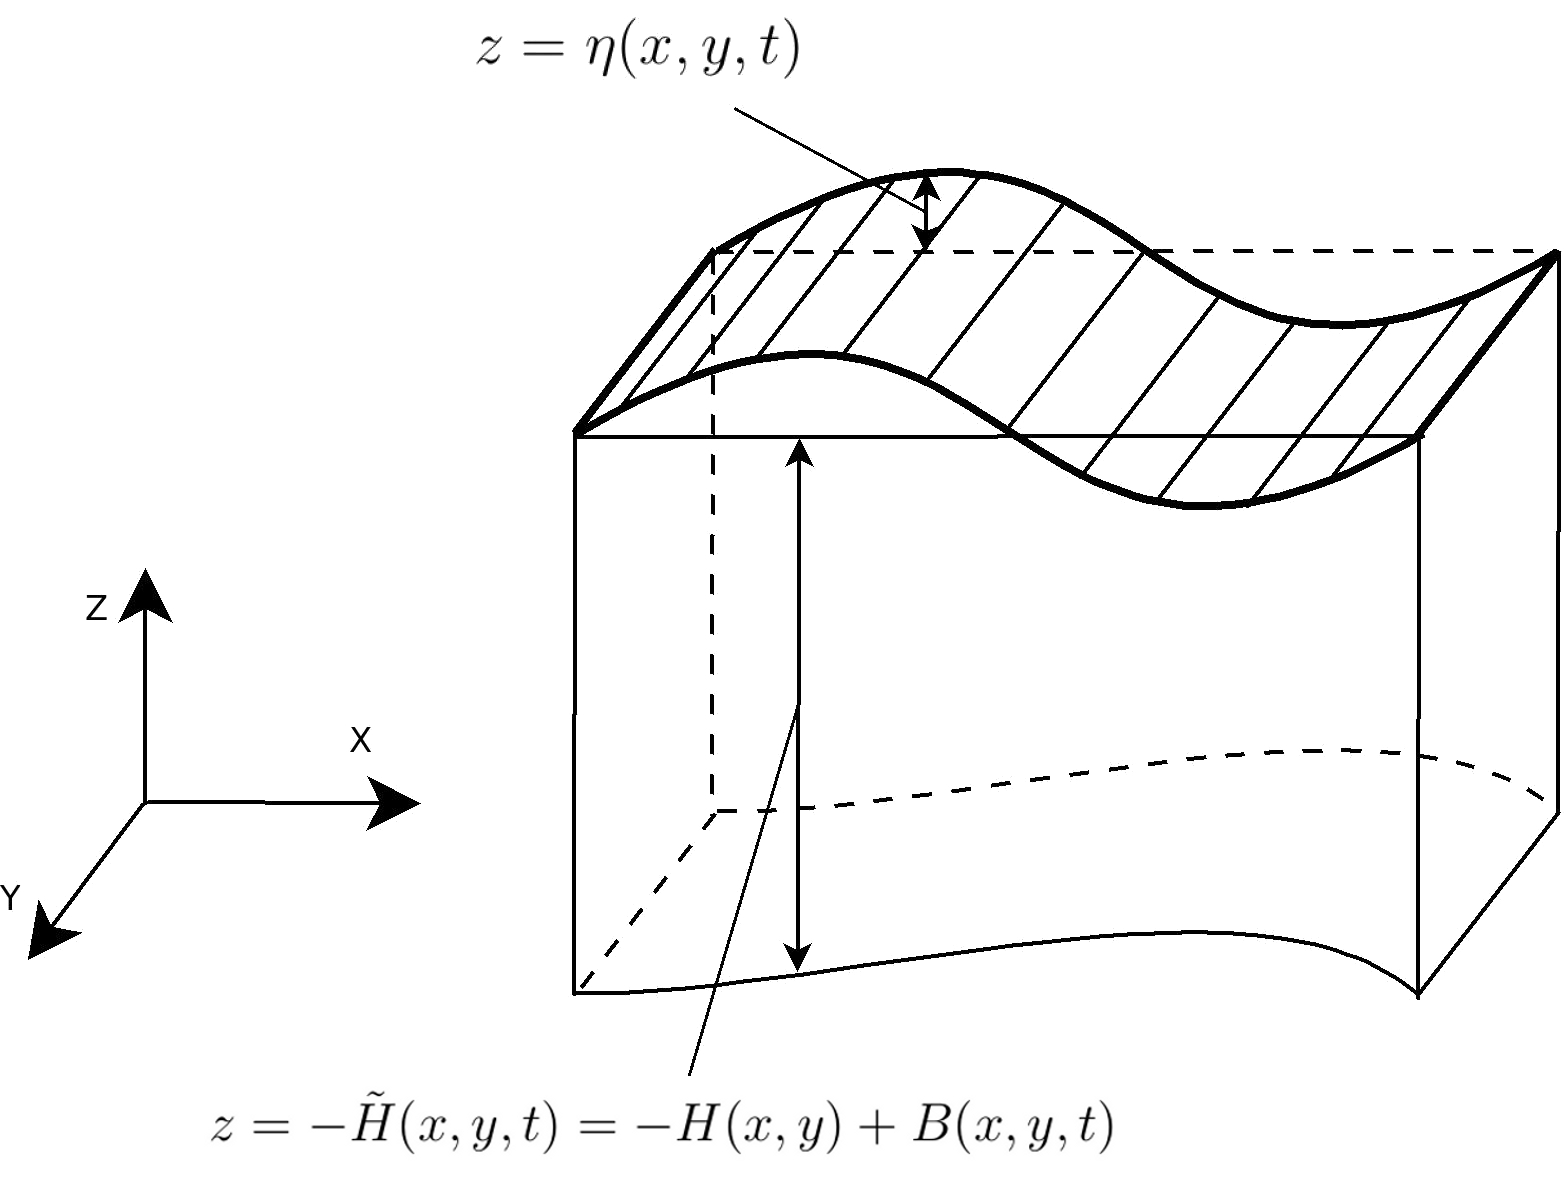
\includegraphics[width=9.5cm]{scheme.jpg}
\end{center}

\end{frame}

%nonlinear equation
\begin{frame}
\frametitle{Постановка задачи}
Уравнения мелкой воды

\begin{gather}
\label{eq:MainVectorForm}
\frac{\partial U}{\partial t}+F_{lin}+F_{nonlin}=\frac{\partial B}{\partial t}\\
\label{eq:UB}
U=\begin{pmatrix}\eta\\u\\v\end{pmatrix}
B=\begin{pmatrix}B(x,y,t)\\0\\0\end{pmatrix}\notag
\end{gather}

\begin{gather}
	\label{eq:Boundary}
	u_0=u(x,y,0)\;v_0=v(x,y,0)\;\eta_0=\eta(x,y,0)\\
	u(x,y,t),v(x,y,t),\eta(x,y,t) \to 0,\; x^2+y^2 \to \infty\notag
\end{gather}

\end{frame}

%nonlinear equation
\begin{frame}
\frametitle{Постановка задачи}
\begin{gather}
\label{eq:FLin}
F_{lin}=\begin{pmatrix}
\frac{\partial ((H-B)u)}{\partial x}+\frac{\partial ((H-B)v)}{\partial y}\\
g\frac{\partial \eta}{\partial x}\\
g\frac{\partial \eta}{\partial y}
\end{pmatrix}\\
\label{eq:FNonLin}
F_{nonlin}=\begin{pmatrix}
0\\
\frac{1}{2}\frac{\partial (u^2)}{\partial x} + v\frac{\partial u}{\partial y}\\
\frac{1}{2}\frac{\partial (v^2)}{\partial y} + u\frac{\partial v}{\partial x}
\end{pmatrix}
\end{gather}
\end{frame}

\begin{frame}
\frametitle{Постановка задачи}
\begin{gather}
\frac{\partial \eta}{\partial t}+\frac{\partial ((H-B)u)}{\partial x}+\frac{\partial ((H-B)v)}{\partial y}=0\notag\\
\frac{\partial u}{\partial t}+\frac{1}{2}\frac{\partial (u^2)}{\partial x} + v\frac{\partial u}{\partial y}+g\frac{\partial \eta}{\partial x}=0\\
\frac{\partial v}{\partial t}+\frac{1}{2}\frac{\partial (v^2)}{\partial y} + u\frac{\partial v}{\partial x}+g\frac{\partial \eta}{\partial y}=0\notag
\end{gather}
\end{frame}

%solving method
\begin{frame}
\frametitle{Метод решения}

\begin{eqnarray}
\label{eq:ApproxMainEq}
\frac{U_{ij}^{n+1}-U_{ij}^{n}}{\tau}+F^{n+1}_{lin}+F^{n+1}_{nonlin}=\frac{B_{ij}^{n+1}-B_{ij}^{n}}{\tau}
\end{eqnarray}

\begin{gather}
\begin{split}
\label{eq:BeginValues}
u_{ij}^0=u_0(x_i,y_i)\;
v_{ij}^0=v_0(x_i,y_i)\;
\eta_{ij}^0=\eta_0(x_i,y_i)
\end{split}
\end{gather}

\begin{gather*}
n=0,1 \ldots N \; i,j=0,\pm 1,\pm 2 \ldots
\end{gather*}
\end{frame}

%solving method
\begin{frame}
\frametitle{Метод решения}

\begin{eqnarray}
\label{eq:ApproxFLin}
F^{n+1}_{lin}=\begin{pmatrix}
\frac{(H_{i+1j}-B_{i+1j}^{n+1})u_{i+1j}^{n+1}-(H_{i-1j}-B_{i-1j}^{n+1})u_{i-1j}^{n+1}}{2h_x}+\\
\frac{(H_{ij+1}-B_{ij+1}^{n+1})v_{ij+1}^{n+1}-(H_{ij-1}-B_{ij-1}^{n+1})v_{ij-1}^{n+1}}{2h_y}\\
g\frac{\eta_{i+1j}^{n+1}-\eta_{i-1j}^{n+1}}{2h_x}\\
g\frac{\eta_{ij+1}^{n+1}-\eta_{ij-1}^{n+1}}{2h_y}
\end{pmatrix}
\end{eqnarray}

\begin{eqnarray}
\label{eq:ApproxFNonlin}
F^{n+1}_{nonlin}=\begin{pmatrix}
0\\
v_{ij}\frac{u_{ij+1}^{n+1}-u_{ij-1}^{n}}{2h_y}+
\frac{1}{2}\frac{(u_{i+1j}^{n+1})^2-(u_{i-1j}^{n})^2}{2h_x}\\
u_{ij}\frac{v_{i+1j}^{n+1}-v_{i-1j}^{n}}{2h_x}+
\frac{1}{2}\frac{(v_{ij+1}^{n+1})^2-(v_{ij-1}^{n})^2}{2h_y}
\end{pmatrix}
\end{eqnarray}
\end{frame}

%boundary conditions
\begin{frame}
\frametitle{Краевые условия}
Для численного решения задачи (\ref{eq:MainVectorForm})-(\ref{eq:Boundary}) необходимо ограничить расчетную область. Существуют способы задания искусcтвенных краевых условий которые в некоторых случаях позволяют выходить волнам из расчетной области без отражений и искажений. Но, к сожалению, они не являются универсальными.
\end{frame}


%boundary conditions
\begin{frame}
\frametitle{Замыкание системы уравнений}
Т.к. границы конечной области ей же и принадлежат, следовательно на них выполняется система  (\ref{eq:MainVectorForm})-(\ref{eq:Boundary}). И тогда для замыкания разностной задачи (\ref{eq:ApproxMainEq})-(\ref{eq:BeginValues}) на границах аппроксимируем систему (\ref{eq:MainVectorForm})-(\ref{eq:Boundary}) внутрь расчетной области.
\end{frame}

%boundary conditions
\begin{frame}
\frametitle{Замыкание системы уравнений}
Пример аппроксимации на $\Gamma_1=\{x=0,y\in[0,1]\}$
\begin{eqnarray}
\label{eq:ApproxFLinGamma1}
F^{n+1}_{lin}=\begin{pmatrix}
\frac{(H_{1j}-B_{1j}^{n+1})u_{1j}^{n+1}-(H_{0j}-B_{0j}^{n+1})u_{0j}^{n+1}}{2h_x}+\\
\frac{(H_{0j+1}-B_{0j+1}^{n+1})v_{0j+1}^{n+1}-(H_{0j-1}-B_{0j-1}^{n+1})v_{0j-1}^{n+1}}{2h_y}\\
g\frac{\eta_{1j}^{n+1}-\eta_{0j}^{n+1}}{2h_x}\\
g\frac{\eta_{0j+1}^{n+1}-\eta_{0j-1}^{n+1}}{2h_y}
\end{pmatrix}
\end{eqnarray}

\begin{eqnarray}
\label{eq:ApproxFNonlinGamma1}
F^{n+1}_{nonlin}=\begin{pmatrix}
0\\
v_{0j}\frac{u_{0j+1}^{n+1}-u_{0j-1}^{n}}{2h_y}+
\frac{1}{2}\frac{(u_{1j}^{n+1})^2-(u_{0j}^{n})^2}{2h_x}\\
u_{0j}\frac{v_{1j}^{n+1}-v_{0j}^{n}}{2h_x}+
\frac{1}{2}\frac{(v_{0j+1}^{n+1})^2-(v_{0j-1}^{n})^2}{2h_y}
\end{pmatrix}
\end{eqnarray}
\end{frame}

%boundary conditions
\begin{frame}
\frametitle{Система уравнений}
В итоге задача (\ref{eq:ApproxMainEq})-(\ref{eq:BeginValues}) с замыканием на границе представляет собой систему нелинейных алгебраических уравнений
\begin{eqnarray}
\label{eq:System}
(A_{lin} + A_{nonlin})\cdot u=f
\end{eqnarray}
Матрица полученной системы уравнений является не самосопряженной, не обладает свойством диагонального преобладания и может быть не знакоопределенной.
\end{frame}

%algorythm
\begin{frame}
\frametitle{Метод неполной аппроксимации}
Для решения системы (\ref{eq:System}) использовался итерационный метод неполной аппроксимации минимальных невязок
\begin{eqnarray}
\label{eq:Alg_first}
u^{k+\frac{1}{2}}=u^k-\tau_{k+1}r^k
\end{eqnarray}
\begin{eqnarray}
\label{eq:Alg_second}
u^{k+1}=u^{k+\frac{1}{2}}-\alpha_{k+1}z_k
\end{eqnarray}
где $\tau$-итерационный параметр,$z^k$ - заданный вектор,$\alpha$-матрица итерационных параметров
\end{frame}

%algorythm
\begin{frame}
\frametitle{Алгоритм решения}
Т.о. для решения задачи (\ref{eq:MainVectorForm})-(\ref{eq:Boundary}) на каждом временном шаге по известному вектору $\{u^n_{ij},v^n_{ij},\eta^n_{ij}\}$ с помощью схемы (\ref{eq:Alg_first})-(\ref{eq:Alg_second}) находится приближенное решение системы (\ref{eq:System}), которое принимается за решение схемы (\ref{eq:ApproxMainEq})-(\ref{eq:BeginValues}) на n+1 слое.
\end{frame}

%results
\begin{frame}
\frametitle{Результаты расчетов}
Нелинейные уравнения
\begin{itemize}
	\item \href{run:video/out_nonlin_gray004.avi}{Движение и накладывание нескольких волн}
	\item \href{run:video/out_model2_standart.avi}{Движение волны с пересечением препятствия в виде усеченного конуса}
	\item \href{run:video/out_model2_map.avi}{Движение волны с пересечением препятствия в виде усеченного конуса(проекция сверху)}
	\item \href{run:video/out_nonlin_exp_buttom.avi}{Движение волны с пересечением препятствия в виде экспоненциального подъема}
\end{itemize}
\end{frame}

%results
\begin{frame}
\frametitle{Результаты расчетов}
Сравнение линейных и нелинейных уравнений при движении над постоянным дном простой формы
\begin{itemize}
	\item \href{run:video/out_lin001.avi}{Движение для линейного случая}
	\item \href{run:video/out_nonlin001.avi}{Движение для нелинейного случая}
	\item \href{run:video/delta001.avi}{Динамика разности}
\end{itemize}
\end{frame}

%results
\begin{frame}
\frametitle{Результаты расчетов}
Сравнение линейных и нелинейных уравнений при движении над постоянным дном с преятствием на границе
\begin{itemize}
	\item \href{run:video/out_lin_100_100.avi}{Движение для линейного случая}
	\item \href{run:video/out_nonlin_100_100.avi}{Движение для нелинейного случая}
	\item \href{run:video/delta_100_100_with_contours.avi}{Динамика разности(с линиями уровня)}
\end{itemize}
\end{frame}

%conclusion
\begin{frame}
\frametitle{Выводы}
\begin{itemize}
	\item Проведены расчеты, демонстрирующие влияние формы дна на движение волны.
	\item Предлагаемый подход решения задачи (\ref{eq:MainVectorForm})-(\ref{eq:Boundary}) с использованием неявных схем и аппроксимации исходной системы уравнений на границе конечной области позволяет находить решение в ней без отражений, как в линейном, так и нелинейном случае.
	\item Нелинейность в (\ref{eq:MainVectorForm})-(\ref{eq:Boundary}) приводит к изменению формы движущихся волн, делает их более ассиметричными. 
\end{itemize}
\end{frame}

%conclusion
\begin{frame}
\frametitle{Конференции}
\begin{itemize}
	\item Одиннадцатая всероссийская конференция <<Прикладные технологии гидроакустики и гидрофизики>>
	\item Всероссийская научно-практическая конференция
<<Научное творчество молодежи>>
	\item X Всероссийская научно-практическая конференция с международным участием <<Информационные технологии
и математическое моделирование>>
\end{itemize}
\end{frame}

\end{document}